\documentclass{beamer}
%\documentclass[handout]{beamer}

\mode<presentation>
{
%  \usetheme{Warsaw}
  % or ...

%  \setbeamercovered{transparent}
  % or whatever (possibly just delete it)
}


\setbeamertemplate{navigation symbols}{}

\usepackage[utf8]{inputenc}
\usepackage[spanish, es-tabla, es-nodecimaldot]{babel}
\usepackage{xcolor}


%\usepackage{times}
%\usepackage[T1]{fontenc}
% Or whatever. Note that the encoding and the font should match. If T1
% does not look nice, try deleting the line with the fontenc.


\title[Intro Prog] % (optional, use only with long paper titles)
{Introducción a la programación}

\subtitle
{Usando Python}

\author[MS]
{Mateo Suster \\ mateosuster@gmail.com}%\inst{1}}
% - Give the names in the same order as the appear in the paper.
% - Use the \inst{?} command only if the authors have different
%   affiliation.

\institute[UNGS] % (optional, but mostly needed)
{
%  \inst{1}%
  Matemática para Economistas III \\ 
  Instituto de Industria\\
  Universidad Nacional de General Sarmiento
%  \and
%  \inst{2}%
%  Department of Theoretical Philosophy\\
%  University of Elsewhere}
% - Use the \inst command only if there are several affiliations.
% - Keep it simple, no one is interested in your street address.
}

\date[] % (optional, should be abbreviation of conference name)
{ \today}



% If you have a file called "university-logo-filename.xxx", where xxx
% is a graphic format that can be processed by latex or pdflatex,
% resp., then you can add a logo as follows:

% \pgfdeclareimage[height=0.5cm]{university-logo}{university-logo-filename}
% \logo{\pgfuseimage{university-logo}}



% Delete this, if you do not want the table of contents to pop up at
% the beginning of each subsection:
%\AtBeginSubsection[]
%{
%  \begin{frame}<beamer>{Outline}
%    \tableofcontents[currentsection,currentsubsection]
%  \end{frame}
%}


% If you wish to uncover everything in a step-wise fashion, uncomment
% the following command: 

%\beamerdefaultoverlayspecification{<+->}


\begin{document}

\begin{frame}
  \titlepage
\end{frame}


\begin{frame}{Antes de arrancar...}
%  \tableofcontents
  % You might wish to add the option [pausesections]
  \begin{block}{Algunas pautas de (esta parte de) la materia}
  \end{block}\pause
  \begin{itemize}
  	\item Todas las preguntas son válidas. \pause 
  	Nadie nace sabiendo. \pause Además, las buenas preguntas son más importantes que las buenas respuestas. \pause
	\item Es importante ir practicando (poco a poco) las cosas que vamos a ir viendo. \pause Esto permitirá evitar la \emph{montaña} de fin de cuatrimestre. \pause (¿Qué necesito para esto?) \pause
	\item Canales de comunicación: \pause Slack (preferentemente) o mail (en casos más puntuales). \pause
	\item Instancias de evaluación \pause
		\begin{itemize}
			\item Participar en Slack (preguntando, respondiendo, debatiendo, "molestando", etc.) \pause
			\item Trabajos Prácticos cuasi-semanales (sin patrón de repetición)\pause
			\item Exámenes Parciales (1 ó 2; fechas a definir)
		\end{itemize}	
  \end{itemize}
\end{frame}



\begin{frame}{Introducción}
%  \tableofcontents
  % You might wish to add the option [pausesections]
  \begin{block}{Info general:}

  \end{block}\pause
  \begin{itemize}
  	\item Objetivo (en principio): programar un sistema de EDOs y graficarlo.
	\pause
	\item Objetivo (en el fondo): generar habilidades que los introduzcan de manera autodidáctica en el mundo de la programación 
	\item ¿Qué es programar? \pause
		\begin{itemize}
			\item Programar $\neq$ saber un lenguaje de programación. \pause
			\item Programar $\neq$ saber usar una computadora. \pause
			\item Frase de Edgar Dijkstra: ``La Ciencia de la Computación no tiene que ver con las computadoras más que la Astronomía con los telescopios''.\pause
		\end{itemize}
	\item ¿Qué lenguajes de programación conocen?\pause
	\item ¿Cuál lenguaje vamos a usar nosotros?\pause
	\begin{itemize}
		\item Respuesta corta: Python. \pause
		\item Respuesta larga: no importa demasiado. Lo importante  son los conocimientos básicos de programación, que son comunes a la mayoría de los lenguajes.%\pause
	\end{itemize}
  \end{itemize}
\end{frame}

\begin{frame}{¿Pero entonces porqué Python?}
\begin{block}{Python actualmente es muy popular} 
	\begin{itemize}
		\item Veamos el \textcolor{blue}{\href{https://www.tiobe.com/tiobe-index/}{Índice Tiobe}}
	\end{itemize}
\end{block}
\begin{center}
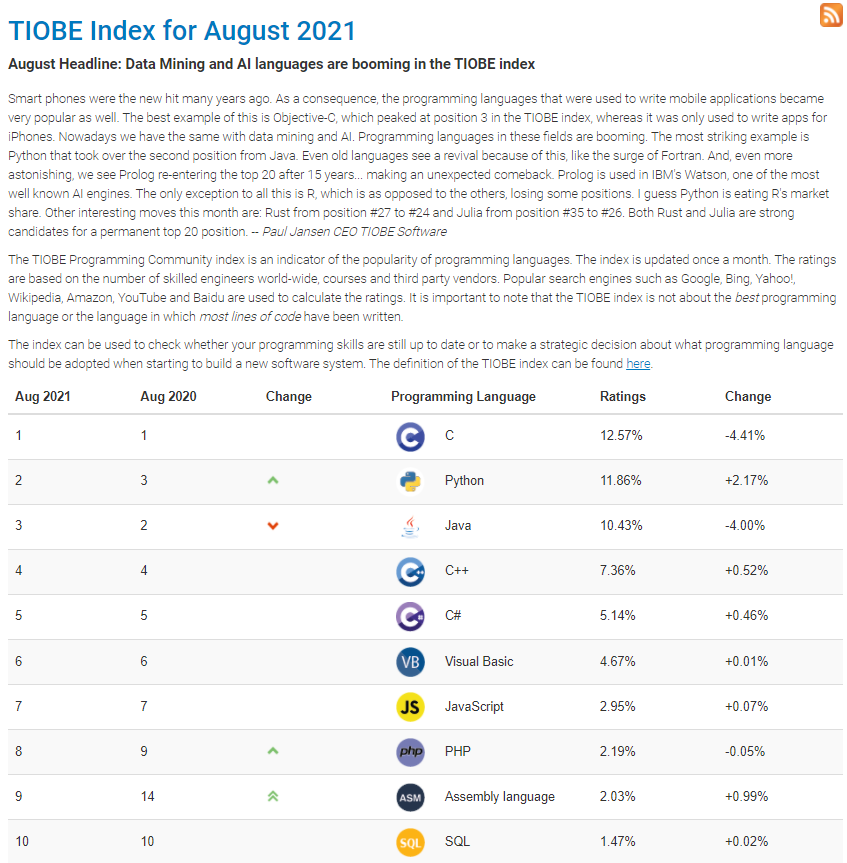
\includegraphics[height=7cm, scale=0.5]{tiobeIndex.png}
\end{center}
\end{frame}

\begin{frame}{¿Sólo por eso elegimos Python?} \pause
Hay otro motivo... \pause
\begin{center}

\includegraphics[height=7cm, scale=0.5]{yoda.png}
\end{center}
\end{frame}


\begin{frame}{Recursos Python}
(\footnotesize Están también en la página \url{https://sebasped.github.io/pythonungs/})
\begin{itemize}
	\item Comunidades:
	\begin{itemize}
		\item \footnotesize\url{http://www.python.org.ar/}
		\item \footnotesize\url{https://argentinaenpython.com/}
		\item \footnotesize\url{https://twitter.com/ChicasProgAR}
		\item \footnotesize\url{https://www.chicasentecnologia.org/}
		\item \footnotesize\url{https://twitter.com/lasdesistemas}
		\item \footnotesize\url{https://www.meetup.com/Buenos-Aires-Python-Meetup/}
		\item \footnotesize\url{https://twitter.com/linuxchixar}
	\end{itemize}\pause
	\item Material, cursos, tutoriales, bibliografía:
	\begin{itemize}
		\item Tutorial de Python para no programadores: \footnotesize\url{http://jjc.freeshell.org/easytut/easytut_es/easytut.html}
		\item \footnotesize\url{http://www.python.org.ar/wiki/AprendiendoPython}
		\item \footnotesize\url{https://argentinaenpython.com/quiero-aprender-python/aprenda-a-pensar-como-un-programador-con-python.pdf}
		\item \footnotesize\url{https://launchpadlibrarian.net/18980633/Python\%20para\%20todos.pdf}
		\item Cursos online (en inglés): coursera, datacamp, udemy, Stanford online, edx, codeacademy, Harvard online, etc.
		%		\item Pilas, colas.
	\end{itemize}\pause
	\item Buscar en internet: hay mucho mucho hecho ya.
\end{itemize}
\end{frame}



\begin{frame}{Elementos básicos programación}
\begin{itemize}
	\item Diferencia entre algoritmo y programa.\pause
	\item Herramientas esenciales:
	\begin{itemize}
		\item Tipos de datos: enteros, reales, strings, etc.% \pause
		\item Variables y expresiones.% \pause
		\item Instrucciones: asignación, condicional, ciclo.%\pause
		\item Funciones, pasajes de parámetros.
	\end{itemize}\pause
	\item Estructuras de datos:
	\begin{itemize}
		\item Listas, arreglos.
		\item Conjuntos, diccionarios.
		\item Pilas, colas.
		\item DataFrames
	\end{itemize}\pause
	\item ¿Cómo se aprende a programar? \pause Programando... no hay manera de aprender algo sin hacerlo.
\end{itemize}
\end{frame}




\begin{frame}{Algoritmo} \pause
\begin{itemize}
	\item Un \emph{algoritmo} es una secuencia de instrucciones. Por ejemplo:\pause
		\begin{enumerate}
		\item Moje el cabello. \pause
		\item Coloque champú.\pause
		\item Masajee suavemente y deje actuar por 2 min.\pause
		\item Enjuague. \pause
		\item Repita el procedimiento desde 1.
		\end{enumerate}
\end{itemize}
\end{frame}

\begin{frame}{Algoritmo}
\begin{itemize}
	\item Una instrucción es una operación que:
	\begin{itemize}
		\item \textcolor{green}{transforma los datos}, o bien
		\item  \textcolor{red}{modifica el flujo de ejecución}
	\end{itemize} \pause
\end{itemize}	
	
		\begin{enumerate}
		\item \textcolor{green}{Moje el cabello.}% \pause
		\item \textcolor{green}{Coloque champú.}% \pause
		\item \textcolor{green}{Masajee suavemente} y \textcolor{red}{deje actuar por 2 min.}%\pause
		\item \textcolor{green}{Enjuague}.
		\item \textcolor{red}{Repita el procedimiento desde 1.}
		\end{enumerate}

\end{frame}




\begin{frame}{Programa} \pause
	\begin{itemize}
	\item Un \emph{programa} es una implementación de un algoritmo en un lenguaje de programación. \pause
		\begin{itemize}
		\item El programa representa al algoritmo en el lenguaje. \pause
		\item Las instrucciones son propias del lenguaje.
		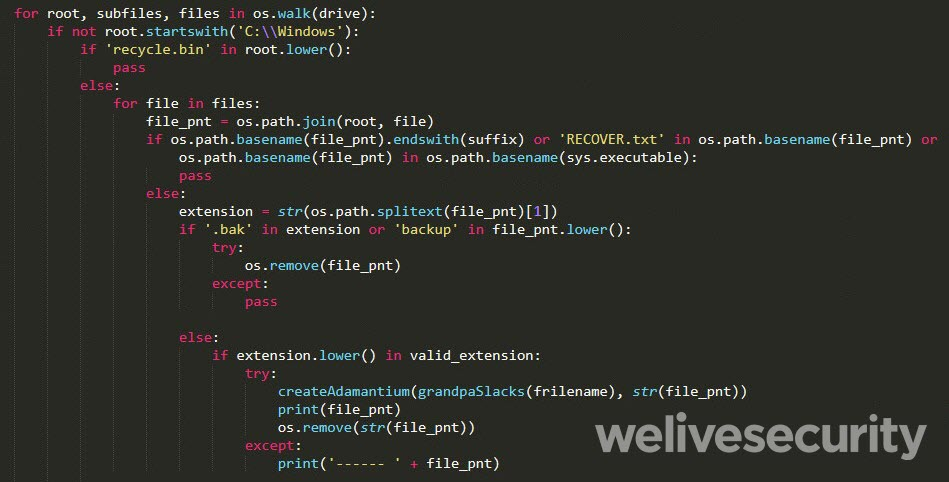
\includegraphics[height=4cm, scale=0.5]{pythonCode.png}						\end{itemize}
	\end{itemize}
\end{frame}


\begin{frame}{Tipos de Datos y Operaciones}
Los programas manipulan \emph{valores} de diferentes \emph{tipos}. Por ejemplo:
\begin{itemize}
	\item 1 es un valor de tipo \textbf{entero} (int).\pause
	\item 2.5 es un valor de tipo \textbf{número ``real''} (float).\pause
	\item ``hola'' es un valor de tipo \textbf{caracter} (string).\pause
	\item ``5'' es un valor de tipo \textbf{caracter} (string).\pause
	\item \'[7.0, 420, “tira de asado”] es dato tipo \textbf{lista} (list).\pause	
	\item False es un valor de tipo \textbf{booleano} (bool).\pause


\begin{itemize}
\item Valores de verdad: Denotan el resultado de una evaluación lógica: los valores “verdadero” (\texttt{True}) y “falso” (\texttt{False})
\end{itemize}
\end{itemize}

Los operaciones son, por ejemplo:
\begin{itemize}
	\item Suma/Resta: 3+4 $\to$ 7.\pause
	\item Se puede sumar strings: probar ``yo y'' + `` mi trasero''.\pause
	\item Producto: 2*8 $\to$ 16.\pause
	\item División: 5/2 $\to$ \pause 2. 
	\item División ``común'': 5/2.0 o 5.0/2 o 5.0/2.0 (i.e. que alguno sea un float).\pause
	\item Resto: 5\%2 $\to$ 1.
	%	\item Práctica para la clase.
\end{itemize}
\end{frame}


\begin{frame}{Colab, Python, IDEs...}
\begin{block}{¿Pero qué se supone son todas esas cosas...?}\pause
\begin{itemize}
	\item Respuesta corta:\pause
		\begin{itemize}
			\item IDE = integrated development environment $\equiv$ entorno de desarrollo integrado.\pause
			\item Google Colab (como Anaconda, un programa usado en anteriores ediciones de este curso) nuclea un montón de paquetes o ``librerías'' (bibliotecas) para usar y no tener que andar reinventando la rueda todo el tiempo.\pause
			\item Google Colab es un entorno que facilita programar en Python. Es una IDE.\pause


		\end{itemize}
	\item Respuesta larga: nada de esto es necesario ni importante para aprender a programar o para codear en Python. Pasa más por gustos personales.\pause
	\begin{itemize}
		\item Por ejemplo, en vez del Anaconda, se podría bajar \textcolor{blue}{\href{https://www.python.org/}{Python}} e ir instalando paquetes.\pause		
%		\item Por ejemplo, en vez del Anaconda, se podría bajar Python (\footnotesize\url{https://www.python.org/}) e ir instalando paquetes.\pause
		\item En vez de Google Colab, para codear se puede usar simplemente un editor de textos, o \textcolor{blue}{\href{https://wiki.python.org/moin/IntegratedDevelopmentEnvironments}{cualquiera de las IDEs existentes}}.
	\end{itemize}
\end{itemize}
\end{block}
\end{frame}

\begin{frame}{Lo que se viene}
\pause
\begin{center}

\includegraphics[height=7cm, scale=0.5]{meme_explosion.png}
\end{center}
\end{frame}


\begin{frame}{Usando Google Colab como IDE para Python}
%(IDE = integrated development environment $\equiv$ entorno de desarrollo integrado).
\begin{block}{Abriendo la IDE...}
\end{block}
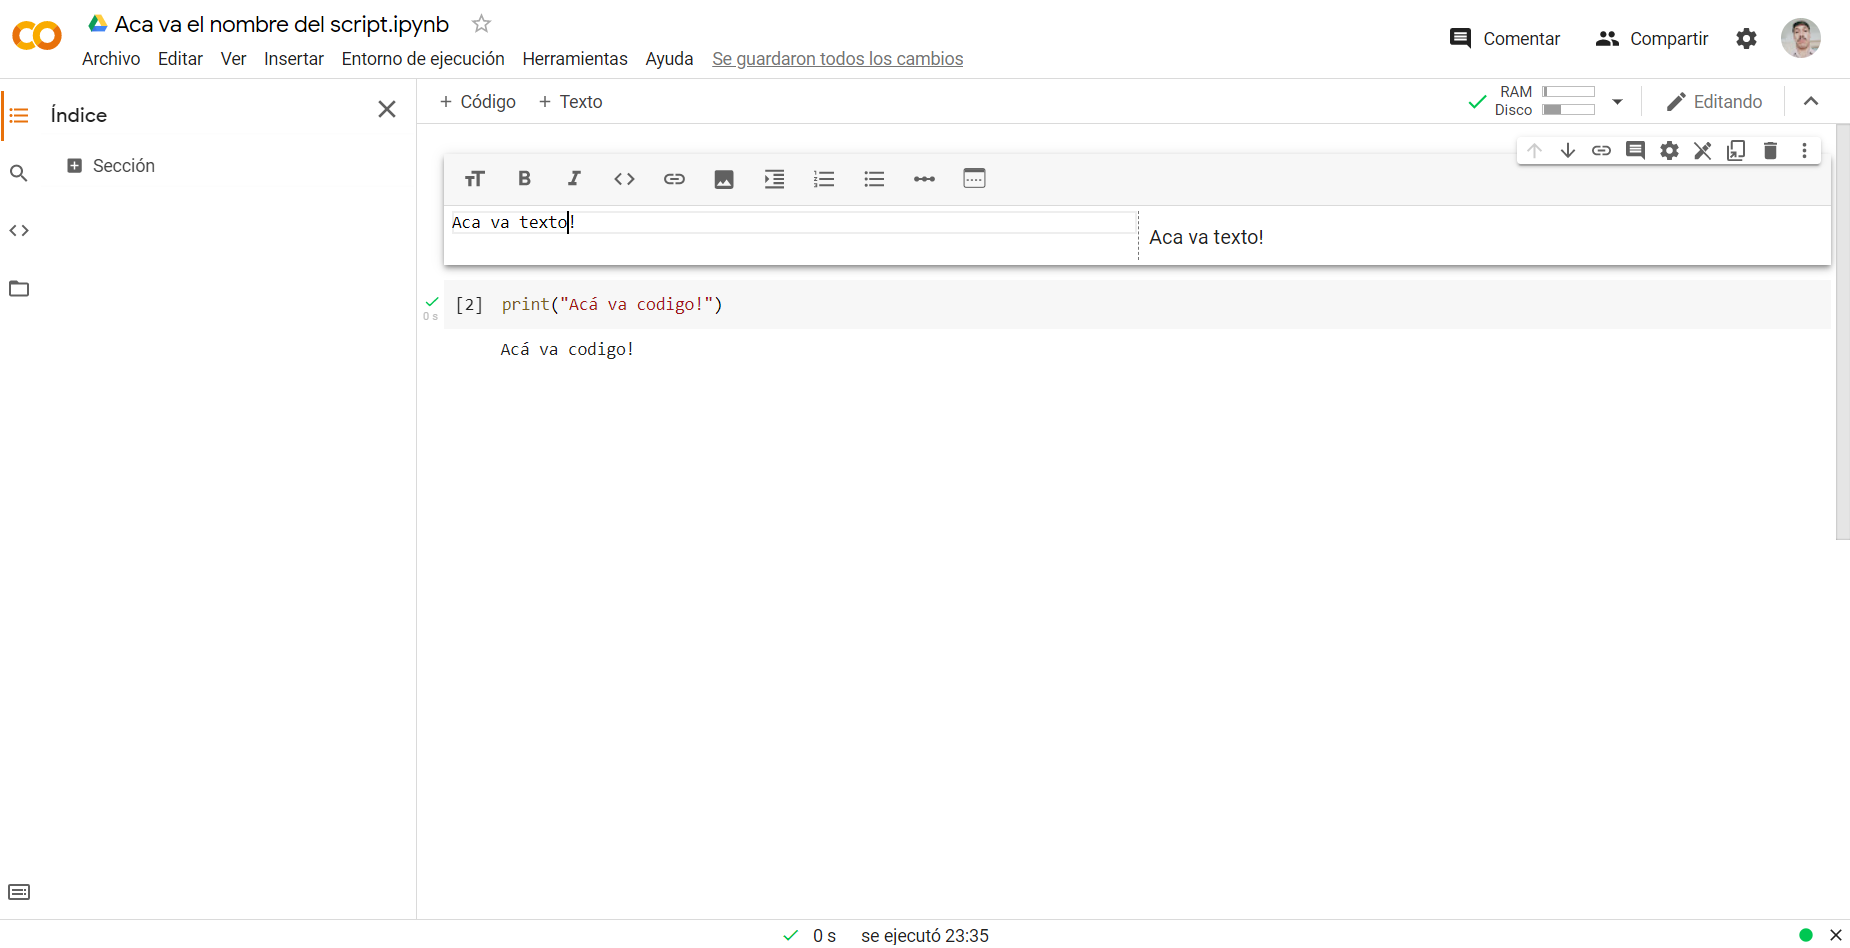
\includegraphics[height=5.5cm]{colab_raw.png}
\end{frame}


\begin{frame}{Tipos de Datos y Comparaciones}
\begin{itemize}
	\item Igualdad: \texttt{i == k}\pause
	\begin{itemize}
		\item Probar \texttt{2 == 3}, \texttt{4 == 4}, \texttt{'a' == 'a'}
	\end{itemize}\pause
	\item Distinto: \texttt{i != k}\pause
	\begin{itemize}
		\item  Probar \texttt{2 != 3}
	\end{itemize}\pause
	\item Menor: \texttt{i$<$k}\pause
	\item Mayor: \texttt{i$>$k}\pause
	\item Menor o igual: \texttt{i$<=$k}\pause
	\item Mayor o igual: \texttt{i$>=$k}
\end{itemize}
\end{frame}

\begin{frame}{Tipos de Datos:  Listas}
Una \emph{lista} es una colección de valores (\textbf{definida entre corchetes}) que se acceden mediante un índice:  \pause
\\~\

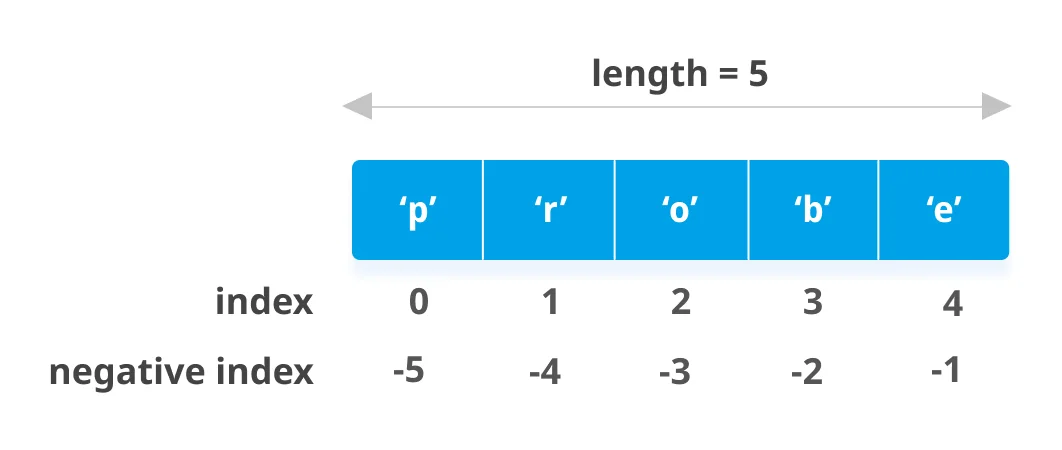
\includegraphics[width=10cm]{lista.png} \pause

\alert{Ojo, el primer elemento tiene índice 0}\pause
\\~
\alert{Y el último elemento tiene índice -1}
\end{frame}


\begin{frame}{Más sobre listas}
Algunos ejemplos de listas y operaciones:
\begin{itemize}
	\item \texttt{$[$2, 3, 5$]$} \pause 
		¿Cuál es el elemento con índice 1?\pause
	\item \texttt{$[$2, 3.5, 'cosita', 8$]$}\pause
	\item \texttt{$[$ $]$} lista vacía.\pause
	\item \texttt{c = $[$2, 3, 5$]$} define una lista de nombre \texttt{c}.
	\item \texttt{$c[i]$} accede o devuelve el elemento con índice i de la lista.\pause
	\item \texttt{len(c)} devuelve la longitud de la lista.\pause
	\item \texttt{c.append(x)} agrega el elemento \texttt{x} al final de la lista \texttt{c}.
	\item Y muchas operaciones más que iremos viendo...
\end{itemize}
\end{frame}

\begin{frame}{En resumen, ¿qué es una lista?}
\pause
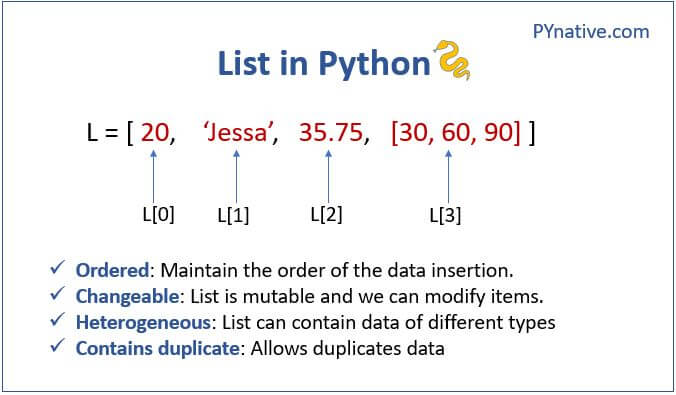
\includegraphics[width=10cm]{python_list.png} 
\end{frame}


\begin{frame}{Variables, expresiones y asignaciones} \pause
\begin{itemize}
	\item Una \textbf{variable} es una dirección de memoria que almacena un valor\pause
		\begin{itemize}
		\item \texttt{b = 3} asigna a la variable \texttt{b} el valor \texttt{3}\pause
		\end{itemize}
	\item Una \textbf{expresión} es una combinación de variables, valores y operadores.\pause
		\begin{itemize}
		\item \texttt{1+1} es una expresión que da como resultado \texttt{2}.\pause
		\end{itemize}
	\item Una \textbf{asignación} es una instrucción que guarda en una variable una expresión.\pause
		\begin{itemize}
		\item \texttt{long = len($[$1,3,'a'$]$)} asigna a la variable long la longitud de la lista $[$1,3,'a'$]$ \pause
		\end{itemize}
\end{itemize}
\alert{Asignación: variable = expresión}
\end{frame}

%\texttt{\begin{frame}{La asignación, nuestra primera instrucción}
%\alert{Asignación: variable = expresión}
%\noindent
%\parbox{2cm}{Bien}%
%\hfill
%
\includegraphics[height=4cm, scale=0.5]{bien.png}
%\end{frame}}


\begin{frame}{La \textbf{asignación}, nuestra primera instrucción}
\alert{VARIABLE = EXPRESIÓN} \pause
\\~
\\~
La asignación almacena el valor de la \emph{expresión} en la dirección en memoria denotada por \emph{variable} \pause
    \begin{columns}
        \begin{column}{.5\textwidth}
			\begin{itemize}
			\item \texttt{x = 1000}
           \item \texttt{x = x + 2}
			\item \texttt{x = y}
			\item \texttt{x = x + y * 22 / 33}
			\end{itemize} \pause
           
        \end{column}
        \begin{column}{.5\textwidth}\raggedleft
            
\includegraphics[scale = 0.3]{bien.png} %width=1cm,height=2cm
        \end{column}
    \end{columns}
\pause
\begin{columns}
        \begin{column}{.5\textwidth}
			\begin{itemize}
			\item \texttt{1000 = x}
           \item \texttt{x + 2 = x}
			\item \texttt{len(x) = 1}
			\end{itemize} \pause
           
        \end{column}
        \begin{column}{.5\textwidth}\raggedleft
            
\includegraphics[scale = 0.3]{mal.png} %width=1cm,height=2cm
        \end{column}
    \end{columns}
    
    
\end{frame}



\begin{frame}{A codea(t)r!}
\begin{block}

\textcolor{blue}{\href{https://colab.research.google.com/drive/1pssmr5FRjDoYxt3-iadaxa-ek3ZmFwPx?usp=sharing}{Link}} a nuestra página de Google Colab	
	
\end{block}
\end{frame}



%\section{Motivation}
%
%\subsection{The Basic Problem That We Studied}
%
%\begin{frame}{Make Titles Informative. Use Uppercase Letters.}{Subtitles are optional.}
%  % - A title should summarize the slide in an understandable fashion
%  %   for anyone how does not follow everything on the slide itself.
%
%  \begin{itemize}
%  \item
%    Use \texttt{itemize} a lot.
%  \item
%    Use very short sentences or short phrases.
%  \end{itemize}
%\end{frame}
%
%\begin{frame}{Make Titles Informative.}
%
%  You can create overlays\dots
%  \begin{itemize}
%  \item using the \texttt{pause} command:
%    \begin{itemize}
%    \item
%      First item.
%      \pause
%    \item    
%      Second item.
%    \end{itemize}
%  \item
%    using overlay specifications:
%    \begin{itemize}
%    \item<3->
%      First item.
%    \item<4->
%      Second item.
%    \end{itemize}
%  \item
%    using the general \texttt{uncover} command:
%    \begin{itemize}
%      \uncover<5->{\item
%        First item.}
%      \uncover<6->{\item
%        Second item.}
%    \end{itemize}
%  \end{itemize}
%\end{frame}
%
%
%\subsection{Previous Work}
%
%\begin{frame}{Make Titles Informative.}
%\end{frame}
%
%\begin{frame}{Make Titles Informative.}
%\end{frame}
%
%
%
%\section{Our Results/Contribution}
%
%\subsection{Main Results}
%
%\begin{frame}{Make Titles Informative.}
%\end{frame}
%
%\begin{frame}{Make Titles Informative.}
%\end{frame}
%
%\begin{frame}{Make Titles Informative.}
%\end{frame}
%
%
%\subsection{Basic Ideas for Proofs/Implementation}
%
%\begin{frame}{Make Titles Informative.}
%\end{frame}
%
%\begin{frame}{Make Titles Informative.}
%\end{frame}
%
%\begin{frame}{Make Titles Informative.}
%\end{frame}
%
%
%
%\section*{Summary}
%
%\begin{frame}{Summary}
%
%  % Keep the summary *very short*.
%  \begin{itemize}
%  \item
%    The \alert{first main message} of your talk in one or two lines.
%  \item
%    The \alert{second main message} of your talk in one or two lines.
%  \item
%    Perhaps a \alert{third message}, but not more than that.
%  \end{itemize}
%  
%  % The following outlook is optional.
%  \vskip0pt plus.5fill
%  \begin{itemize}
%  \item
%    Outlook
%    \begin{itemize}
%    \item
%      Something you haven't solved.
%    \item
%      Something else you haven't solved.
%    \end{itemize}
%  \end{itemize}
%\end{frame}
%
%
%
%% All of the following is optional and typically not needed. 
%\appendix
%\section<presentation>*{\appendixname}
%\subsection<presentation>*{For Further Reading}
%
%\begin{frame}[allowframebreaks]
%  \frametitle<presentation>{For Further Reading}
%    
%  \begin{thebibliography}{10}
%    
%  \beamertemplatebookbibitems
%  % Start with overview books.
%
%  \bibitem{Author1990}
%    A.~Author.
%    \newblock {\em Handbook of Everything}.
%    \newblock Some Press, 1990.
% 
%    
%  \beamertemplatearticlebibitems
%  % Followed by interesting articles. Keep the list short. 
%
%  \bibitem{Someone2000}
%    S.~Someone.
%    \newblock On this and that.
%    \newblock {\em Journal of This and That}, 2(1):50--100,
%    2000.
%  \end{thebibliography}
%\end{frame}

\end{document}



